% Provenance (never printed): see sources/outline_sources.md (Year 1: continental
% rifting and break-up; passive-margin structure; fast and slow ridges; the depth--age
% law of the ocean floor; transform faults). Curve from figdata/bachelor-1/depth_age.py;
% exercise and problem values in the Book 3 scratch calculator calc/ch13.py; the
% coordinates of the margin schematic from calc/fig13_margin.py.
\chapter{Fosas, dorsales y márgenes pasivos}\label{ch:b1:rifts-ridges-margins}

En septiembre de 2005 se abrió el suelo del desierto de Afar, en el noreste de Etiopía. En tres semanas un tramo del rift de unos
\qty{60}{km} de longitud se ensanchó hasta \qty{8}{m}, y unos \qty{2.5}{km^3} de magma subieron a la grieta desde abajo. Las placas allí
se separan a unos \qty{18}{mm} al año: la crisis liberó, en unas semanas, el estiramiento de unos cuatro siglos. Afar es un continente
que se rompe; a unos cientos de kilómetros al norte, el mar Rojo es un océano joven cuyo fondo ya está hecho como el del Atlántico, y el
Atlántico Sur fue un rift así antes de abrirse, hace unos 120 millones de años. Este capítulo sigue el nacimiento de un océano: el
estiramiento de un continente, su ruptura, los dos márgenes pasivos que quedan, la dorsal que construye el fondo oceánico y el hundimiento
lento de ese fondo al enfriarse.
% ledger: wright:afar, morvel:ar-nb (18.5 mm/yr at 12.3 N, 40.6 E, computed with euler_velocities.py), heine:fit

\begin{recall}
Las placas son la \omterm{def:b1:heat-budget:boundary-layer}{capa límite térmica} superior del \omterm{def:b1:layered-earth:layers}{manto}; bajo los océanos un semiespacio que se enfría las describe, y sus isotermas se
hunden como la raíz cuadrada de la edad (\cref{ch:b1:heat-budget}). Las columnas de roca en equilibrio isostático tienen la misma masa por
unidad de área sobre una \omterm{def:b1:isostasy-gravity:isostasy}{profundidad de compensación} (\cref{ch:b1:isostasy-gravity}). Las placas giran alrededor de \omterm{def:b1:plate-kinematics:euler-pole}{polos de Euler}, las
dorsales se expanden a velocidades leídas en las anomalías magnéticas, y las transformantes yacen sobre \omterm{def:b1:spherical-astronomy:spherical-triangle}{círculos menores} alrededor del polo
(\cref{ch:b1:plate-kinematics}). El salto y el desplazamiento de una falla se definieron en \cref{ch:b1:cross-sections}; una falla normal es
una falla inclinada cuyo bloque superior ha bajado (libro 2, año 11).
\end{recall}

\section{Rifting continental}

Un continente estirado por fuerzas en sus bordes no se adelgaza de forma uniforme. Su \omterm{def:b1:layered-earth:layers}{corteza} superior frágil se rompe a lo largo de fallas
normales, y los bloques entre ellas se hunden e inclinan; por debajo, la \omterm{def:b1:layered-earth:layers}{corteza} inferior más caliente y el \omterm{def:b1:layered-earth:layers}{manto} fluyen.

\begin{definition}[Rift continental, graben, semigraben]\label{def:b1:rifts-ridges-margins:rift}
Un \emph{rift continental}\index{rift continental} es una zona larga y estrecha donde un continente se está estirando: una depresión
limitada por fallas normales, con terremotos y, a menudo, volcanes. Un \emph{graben}\index{graben} es un bloque hundido entre dos fallas
normales que buzan una hacia la otra. Un \emph{semigraben}\index{semigraben} es un bloque hundido e inclinado contra una sola falla
normal mayor, la falla de borde, por un solo lado.
\end{definition}

La mayoría de las cuencas de rift son cadenas de semigrábenes. Sus fallas de borde se transmiten el desplazamiento unas a otras mediante
rampas de relevo, y el lado de la falla de borde suele alternar de un segmento al siguiente. El bloque colgante de cada falla de borde se
inclina hacia ella, y la cuenca se llena más deprisa allí: el sedimento más grueso se acumula contra la falla, mientras que el bloque
yacente se eleva formando el hombro del rift.

El estiramiento horizontal que transmite una falla es su \omterm{def:b1:cross-sections:throw}{salto horizontal}. Una falla normal plana de salto $h$ y \omterm{def:b1:geological-maps:attitude}{buzamiento} $\delta$ tiene
un \omterm{def:b1:cross-sections:throw}{salto horizontal} $h/\tan\delta$ (\cref{ch:b1:cross-sections}); sumando los \omterm{def:b1:cross-sections:throw}{saltos horizontales} de las fallas a través de una sección del
rift se obtiene el estiramiento de la \omterm{def:b1:layered-earth:layers}{corteza} frágil. Cómo se adelgaza toda la \omterm{def:b1:layered-earth:lithosphere}{litosfera} al estirarse, y por qué se hunde después, se
cuantifica en el libro de segundo año universitario; aquí se miden las fallas, y su suma se compara con el movimiento de las placas.

\begin{omfigure}
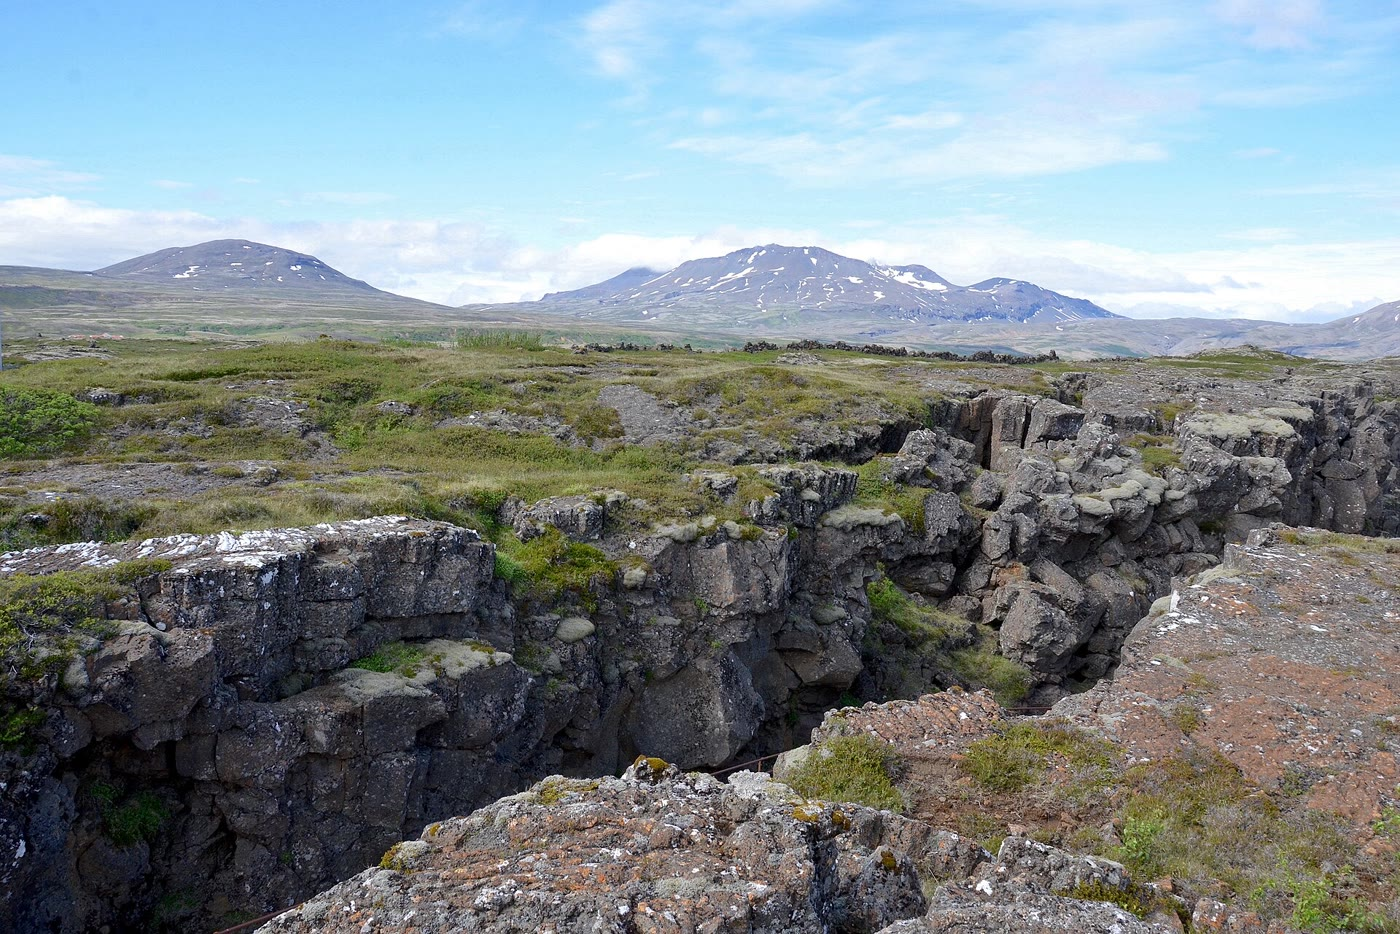
\includegraphics[width=0.8\linewidth]{images/book3/b1-thingvellir-fissure.jpg}

\par\smallskip{\small Una fisura abierta en el suelo de lava del valle de rift de Þingvellir, en el suroeste de Islandia, donde la
dorsal medioatlántica emerge. Los flujos de basalto del fondo del valle están cortados por fisuras abiertas paralelas al rift. Fotografía:
Olga Ernst, CC~BY-SA~4.0 (Wikimedia Commons).}
\label{fig:b1:rifts-ridges-margins:thingvellir}
\end{omfigure}
% ledger: commons:thingvellir

\subsection*{Rifts volcánicos y rifts pobres en magma}

Los rifts difieren en la cantidad de magma que reciben. En un rift \emph{pobre en magma} el estiramiento lo absorben las fallas, y la
\omterm{def:b1:layered-earth:layers}{corteza} se adelgaza a medida que los bloques se deslizan. En un rift volcánico el magma toma el relevo: los diques se intruyen en la \omterm{def:b1:layered-earth:layers}{corteza}
a lo largo del eje, abriendo cada uno el rift en su propio espesor, y las lavas inundan la superficie. El rift de África Oriental muestra
ambos, uno junto al otro: su rama oriental es fuertemente volcánica, mientras que la occidental lo es menos y tiene cuencas sedimentarias
profundas, ocupadas por lagos como el Tanganica y limitadas por fallas.
% ledger: roberts:ear

Ambas ramas empezaron a formarse hace unos 25 millones de años, y el rift divide la placa africana en una placa nubia al oeste y una
placa somalí al este. Desde la \omterm{def:b1:plate-kinematics:triple-junction}{unión triple} de Afar corre hacia el sur, en dos ramas alrededor del antiguo, grueso y frío cratón de
Tanzania. Su movimiento es lento: calculado a partir de los vectores de placa de Somalia y Nubia, cada uno medido respecto de la placa
antártica, Somalia se aleja de Nubia a \qty{6.0}{mm.yr^{-1}} hacia \ang{105} en el centro de Etiopía (\ang{8.5}\,N, \ang{39.5}\,E), y a
\qty{5.1}{mm.yr^{-1}} en el ecuador. Muchos terremotos del rift muestran fallamiento normal.
% ledger: roberts:ear, morvel:sm-an, morvel:nb-an (SM-NB from SM-AN minus NB-AN, computed with figdata/bachelor-1/euler_velocities.py)

En Afar, en el extremo norte, el rift se encuentra con el mar Rojo y el golfo de Adén. La mayor parte de los basaltos de inundación de
Etiopía brotó allí hace unos 30 millones de años, en un millón de años o menos, y el magma no ha dejado de llegar desde entonces: coladas
en la superficie, intrusiones en la \omterm{def:b1:layered-earth:layers}{corteza} y material nuevo añadido debajo, tanto que la \omterm{def:b1:layered-earth:layers}{corteza} intruida ha mantenido su espesor durante
las primeras etapas del rifting. La crisis de 2005 muestra cómo se abre un rift así: no de forma continua, sino a golpes, cada uno un dique
de metros de anchura intruido en días o semanas. Como las placas se separan allí a unos \qty{18}{mm.yr^{-1}}, el dique de \qty{8}{m} de 2005
equivale a unos 440 años de estiramiento.
% ledger: hofmann:traps, bastow:afar, wright:afar, morvel:ar-nb (rate computed with euler_velocities.py)

\section{Ruptura y márgenes pasivos}

Si el estiramiento continúa, la \omterm{def:b1:layered-earth:layers}{corteza} continental se adelgaza hasta desaparecer, el \omterm{def:b1:layered-earth:layers}{manto} asciende bajo el rift y se funde al subir, y se
forma entre las dos mitades del continente la primera \omterm{def:b1:rifts-ridges-margins:oceanic-crust}{corteza oceánica}. Ese momento es la \emph{ruptura}. A partir de entonces las placas
se separan en una dorsal en el centro de un nuevo océano, y los dos bordes del continente, llevados lejos de la dorsal, dejan de ser
fronteras de placas.

\begin{definition}[Margen pasivo, transición océano--continente, discordancia de ruptura]\label{def:b1:rifts-ridges-margins:passive-margin}
Un \emph{margen pasivo}\index{margen pasivo} es el borde de un continente formado por rifting que ya no es una frontera de placas: el
continente y el fondo oceánico contiguo pertenecen a la misma placa. La \emph{transición océano--continente}\index{transición océano--continente}
es la zona del margen, de kilómetros a decenas de kilómetros de ancho, entre la \omterm{def:b1:layered-earth:layers}{corteza} continental adelgazada y la \omterm{def:b1:rifts-ridges-margins:oceanic-crust}{corteza oceánica} normal.
La \emph{discordancia de ruptura}\index{discordancia de ruptura} es la \omterm{def:b1:cross-sections:unconformity}{discordancia} que separa los sedimentos depositados en las cuencas de
rift, inclinados con sus bloques, de los sedimentos no perturbados depositados sobre el margen después de la ruptura.
\end{definition}

Los márgenes pasivos bordean la mayor parte del Atlántico, el océano Ártico y el océano Índico occidental, y casi todas las costas de
África, Australia, Groenlandia y la India. El margen oriental de Norteamérica y el margen noroccidental de África fueron los dos lados de
un mismo rift: son márgenes \emph{conjugados}. Su perfil es la conocida sucesión del fondo oceánico junto a tierra: plataforma continental,
talud, elevación continental y llanura abisal. Bajo la plataforma y el talud yace la \omterm{def:b1:layered-earth:layers}{corteza} continental adelgazada, cortada por fallas
normales que buzan hacia el océano, con sus bloques rotados enterrados bajo los sedimentos.

\begin{omfigure}
\begin{tikzpicture}[x=0.95cm, y=0.9cm, font=\scriptsize]
% (a) continental rift: half-grabens on east-dipping faults; coordinates from calc/fig13_margin.py
\begin{scope}
\fill[green!25!gray!45] (0,-2) -- (3,-2) -- (6,-1.75) -- (9,-2) -- (12,-2) -- (12,-2.5) -- (0,-2.5) -- cycle;
\fill[orange!22] (0,0) -- (3.5,0) -- (3.931,-0.8) -- (4.75,-0.25) -- (5.05,-0.7) -- (6,-0.2) -- (6.223,-0.55) -- (7.25,-0.15) -- (7.402,-0.4) -- (8.6,0) -- (12,0) -- (12,-2) -- (9,-2) -- (6,-1.75) -- (3,-2) -- (0,-2) -- cycle;
\fill[yellow!45] (3.565,-0.12) -- (3.931,-0.8) -- (4.75,-0.25) -- (4.75,-0.12) -- cycle;
\fill[yellow!45] (4.75,-0.12) -- (4.75,-0.25) -- (5.05,-0.7) -- (6,-0.2) -- (6,-0.12) -- cycle;
\fill[yellow!45] (6,-0.12) -- (6,-0.2) -- (6.223,-0.55) -- (7.25,-0.15) -- (7.25,-0.12) -- cycle;
\fill[yellow!45] (7.25,-0.12) -- (7.25,-0.15) -- (7.402,-0.4) -- (8.241,-0.12) -- cycle;
\draw (0,0) -- (3.5,0) -- (3.931,-0.8) -- (4.75,-0.25) -- (5.05,-0.7) -- (6,-0.2) -- (6.223,-0.55) -- (7.25,-0.15) -- (7.402,-0.4) -- (8.6,0) -- (12,0);
\draw[contact] (0,-2) -- (3,-2) -- (6,-1.75) -- (9,-2) -- (12,-2);
\draw[fault] (3.5,0) -- (4.2,-1.3);
\draw[fault] (4.75,-0.25) -- (5.45,-1.3);
\draw[fault] (6,-0.2) -- (6.7,-1.3);
\draw[fault] (7.25,-0.15) -- (7.95,-1.3);
\node[anchor=west, font=\small\bfseries] at (0,0.75) {(a) rift continental};
\node[anchor=south] at (2.2,0) {hombro del rift};
\node[anchor=south, align=center] at (6.3,0) {semigrábenes rellenos de sedimento};
\draw[-{Stealth[length=3pt]}] (2.6,-0.75) node[anchor=east] {falla de borde} -- (3.75,-0.5);
\node at (9.8,-1.0) {corteza continental};
\node at (10.3,-2.25) {manto};
\node at (6,-2.18) {Moho elevado bajo el rift};
\end{scope}
% (b) break-up: conjugate halves, the first oceanic crust between them
\begin{scope}[yshift=-3.6cm]
\fill[omSea!35] (2.8,0) -- (9.2,0) -- (9.2,-1.3) -- (2.8,-1.3) -- cycle;
\fill[green!25!gray!45] (0,-2) -- (2.5,-2) -- (5.5,-1.3) -- (6.5,-1.3) -- (9.5,-2) -- (12,-2) -- (12,-2.5) -- (0,-2.5) -- cycle;
\fill[orange!22] (0,0) -- (2.8,0) -- (3.146,-0.75) -- (3.8,-0.3) -- (4.13,-0.85) -- (4.7,-0.45) -- (5.053,-0.95) -- (5.5,-1) -- (5.5,-1.3) -- (2.5,-2) -- (0,-2) -- cycle;
\fill[orange!22] (12,0) -- (9.2,0) -- (8.854,-0.75) -- (8.2,-0.3) -- (7.87,-0.85) -- (7.3,-0.45) -- (6.947,-0.95) -- (6.5,-1) -- (6.5,-1.3) -- (9.5,-2) -- (12,-2) -- cycle;
\fill[lith basalt] (5.5,-1) -- (6.5,-1) -- (6.5,-1.3) -- (5.5,-1.3) -- cycle;
\draw (0,0) -- (2.8,0) -- (3.146,-0.75) -- (3.8,-0.3) -- (4.13,-0.85) -- (4.7,-0.45) -- (5.053,-0.95) -- (5.5,-1) -- (6.5,-1) -- (6.947,-0.95) -- (7.3,-0.45) -- (7.87,-0.85) -- (8.2,-0.3) -- (8.854,-0.75) -- (9.2,0) -- (12,0);
\draw[contact] (0,-2) -- (2.5,-2) -- (5.5,-1.3) -- (6.5,-1.3) -- (9.5,-2) -- (12,-2);
\draw[omSea!70!black] (2.8,0) -- (9.2,0);
\draw[fault] (2.8,0) -- (3.4,-1.3);
\draw[fault] (3.8,-0.3) -- (4.4,-1.3);
\draw[fault] (4.7,-0.45) -- (5.3,-1.3);
\draw[fault] (9.2,0) -- (8.6,-1.3);
\draw[fault] (8.2,-0.3) -- (7.6,-1.3);
\draw[fault] (7.3,-0.45) -- (6.7,-1.3);
\draw[omRidge, very thick, -{Stealth[length=3pt]}] (6,-2.3) -- (6,-1.45);
\node[anchor=west, font=\small\bfseries] at (0,0.75) {(b) ruptura};
\node[anchor=south] at (6,0) {el mar inunda el rift};
\node[anchor=west] at (6.15,-2.1) {el manto sube y se funde};
\node[anchor=south, fill=white, fill opacity=0.8, text opacity=1, inner sep=1pt, align=center] at (6,-0.85) {primera\\corteza oceánica};
\node at (1.4,-1.0) {bloques inclinados};
\node at (10.6,-1.0) {bloques inclinados};
\node at (1.4,-2.25) {manto};
\end{scope}
% (c) one passive margin after drift
\begin{scope}[yshift=-7.4cm]
\fill[omSea!35] (1.2,0.3) -- (12,0.3) -- (12,-1.2) -- (8.2,-1.15) -- (6.4,-0.9) -- (4.6,0.1) -- cycle;
\fill[green!25!gray!45] (0,-2.3) -- (2,-2.3) -- (5.9,-1.8) -- (6.7,-2.1) -- (12,-2.1) -- (12,-2.7) -- (0,-2.7) -- cycle;
\fill[orange!22] (0,0.3) -- (1.2,0.3) -- (2.2,0) -- (3,-0.25) -- (3.259,-0.95) -- (4,-0.55) -- (4.286,-1.15) -- (4.9,-0.85) -- (5.233,-1.35) -- (5.9,-1.55) -- (5.9,-1.8) -- (2,-2.3) -- (0,-2.3) -- cycle;
\fill[pattern=crosshatch dots, pattern color=green!40!black] (5.9,-1.55) -- (6.4,-1.75) -- (6.7,-2.1) -- (5.9,-1.8) -- cycle;
\fill[lith basalt] (6.4,-1.75) -- (12,-1.75) -- (12,-2.1) -- (6.7,-2.1) -- cycle;
\fill[yellow!45] (3,-0.25) -- (3.259,-0.95) -- (4,-0.55) -- cycle;
\fill[yellow!45] (4,-0.55) -- (4.286,-1.15) -- (4.9,-0.85) -- cycle;
\fill[yellow!45] (4.9,-0.85) -- (5.233,-1.35) -- (5.9,-1.55) -- (5.9,-1.45) -- cycle;
\fill[yellow!15] (1.2,0.3) -- (4.6,0.1) -- (6.4,-0.9) -- (8.2,-1.15) -- (12,-1.2) -- (12,-1.75) -- (6.4,-1.75) -- (5.9,-1.55) -- (5.9,-1.45) -- (4.9,-0.85) -- (4,-0.55) -- (3,-0.25) -- (2.2,0) -- cycle;
\draw[black!45] (2.4,0.12) -- (4.8,-0.1) -- (6.6,-1.05) -- (8.4,-1.27) -- (12,-1.31);
\draw (1.2,0.3) -- (4.6,0.1) -- (6.4,-0.9) -- (8.2,-1.15) -- (12,-1.2);
\draw[omSea!70!black] (1.2,0.3) -- (12,0.3);
\draw[unconformity] (2.2,0) -- (3,-0.25) -- (4,-0.55) -- (4.9,-0.85) -- (5.9,-1.45);
\draw (3.259,-0.95) -- (4,-0.55) (4.286,-1.15) -- (4.9,-0.85) (5.233,-1.35) -- (5.9,-1.55) -- (6.4,-1.75) -- (12,-1.75);
\draw[contact] (0,-2.3) -- (2,-2.3) -- (5.9,-1.8) -- (6.7,-2.1) -- (12,-2.1);
\draw[fault] (3,-0.25) -- (3.5,-1.6);
\draw[fault] (4,-0.55) -- (4.5,-1.6);
\draw[fault] (4.9,-0.85) -- (5.4,-1.6);
\node[anchor=west, font=\small\bfseries] at (0,0.95) {(c) margen pasivo};
\node[anchor=south] at (3.4,0.25) {plataforma};
\node[anchor=south west] at (5.6,-0.45) {talud};
\node[anchor=south] at (8.4,-1.12) {elevación};
\node[anchor=south] at (10.6,-1.17) {llanura abisal};
\node[anchor=south] at (10.6,-0.1) {océano};
\node at (9.8,-1.53) {sedimentos postrift};
\node[fill=white, fill opacity=0.8, text opacity=1, inner sep=1pt, align=center] (bu) at (1.0,-0.6) {discordancia\\de ruptura};
\draw[-{Stealth[length=3pt]}] (bu.east) -- (2.55,-0.16);
\node[fill=white, fill opacity=0.8, text opacity=1, inner sep=1pt, align=center] (sr) at (1.6,-1.35) {sedimentos\\sinrift};
\draw[-{Stealth[length=3pt]}] (sr.east) -- (3.45,-0.75);
\node at (1.3,-1.98) {corteza continental};
\draw[decorate, decoration={brace, amplitude=3pt, mirror}] (5.9,-2.17) -- (6.7,-2.17) node[midway, below=3pt, align=center] {transición\\océano--continente};
\node[anchor=west, fill=white, fill opacity=0.85, text opacity=1, inner sep=1pt] at (8.6,-1.93) {corteza oceánica};
\node at (3.6,-2.5) {manto};
\end{scope}
\end{tikzpicture}

\par\smallskip{\small Del rift al \omterm{def:b1:rifts-ridges-margins:passive-margin}{margen pasivo} (dibujos, no a escala; las alturas están exageradas). (a) La \omterm{def:b1:layered-earth:layers}{corteza} superior frágil se
rompe a lo largo de fallas normales; los bloques se inclinan formando semigrábenes que se rellenan de sedimento, y el \omterm{def:b1:layered-earth:discontinuity}{Moho} sube bajo la
\omterm{def:b1:layered-earth:layers}{corteza} adelgazada. (b) En la ruptura la \omterm{def:b1:layered-earth:layers}{corteza} continental queda cortada del todo; el mar inunda el rift y se forma la primera \omterm{def:b1:rifts-ridges-margins:oceanic-crust}{corteza
oceánica}. (c) Uno de los dos márgenes, llevado lejos de la dorsal: sus bloques inclinados y sus sedimentos yacen bajo la \omterm{def:b1:rifts-ridges-margins:passive-margin}{discordancia de
ruptura}, enterrados por los sedimentos postrift de la plataforma, el talud y la elevación continental.}
\label{fig:b1:rifts-ridges-margins:margin}
\end{omfigure}

\subsection*{Dos tipos de margen}

Los márgenes heredan el carácter de su rift. En los márgenes \emph{pobres en magma}, como los de Iberia y Terranova, las secciones sísmicas
muestran bloques rotados cuyas capas buzan hacia el continente; en algunos lugares la \omterm{def:b1:rifts-ridges-margins:passive-margin}{transición océano--continente} está formada por
peridotita del \omterm{def:b1:layered-earth:layers}{manto}, llevada hasta el fondo del mar y alterada por el agua de mar hasta serpentinita. En los márgenes \emph{volcánicos},
como los del centro de Noruega, de Groenlandia oriental, de Namibia y de Brasil, la transición está construida de basalto: pilas de
coladas que buzan hacia el océano, los reflectores que buzan hacia el mar de las secciones sísmicas, y debajo de ellas una \omterm{def:b1:layered-earth:layers}{corteza}
inferior en la que las ondas P viajan inusualmente rápido, magma añadido bajo la \omterm{def:b1:layered-earth:layers}{corteza} en la ruptura. Los márgenes volcánicos se
hunden poco durante la ruptura.

\begin{inthefield}[Encontrar el borde de un continente]
La \omterm{def:b1:rifts-ridges-margins:passive-margin}{transición océano--continente} yace bajo kilómetros de agua y sedimento, y solo la geofísica la localiza, habitualmente con varios
métodos a la vez. La reflexión sísmica muestra los bloques inclinados, la \omterm{def:b1:rifts-ridges-margins:passive-margin}{discordancia de ruptura} y, cuando la señal llega lo bastante
profundo, el \omterm{def:b1:layered-earth:discontinuity}{Moho}. La refracción sísmica de gran ángulo mide las velocidades de las ondas P a través de la \omterm{def:b1:layered-earth:layers}{corteza}, que difieren entre
\omterm{def:b1:layered-earth:layers}{corteza} continental y oceánica. Los datos gravimétricos, invertidos para obtener la profundidad del \omterm{def:b1:layered-earth:discontinuity}{Moho}, dan el espesor de la \omterm{def:b1:layered-earth:layers}{corteza}.
Las franjas magnéticas del fondo oceánico se detienen donde empieza la \omterm{def:b1:layered-earth:layers}{corteza} continental, magnéticamente tranquila.
\end{inthefield}

Después de la ruptura, un margen se hunde. Durante el rifting la \omterm{def:b1:layered-earth:lithosphere}{litosfera} se adelgazó y se calentó; llevada lejos de la dorsal, se enfría
y se contrae, como el fondo oceánico contiguo, y el espacio que se abre sobre ella se llena con la cuña de sedimentos postrift, cuyo peso la
hunde aún más. La mitad fría de esta historia se cuenta en \cref{sec:b1:rifts-ridges-margins:depth-age}; el peso de los sedimentos es el
tema de \cref{ch:b1:diagenesis-basins}.

\section{Dorsales rápidas y lentas}

Una vez nacido, el océano crece en su dorsal. Las dorsales se expanden a velocidades muy distintas: las velocidades medidas durante los
últimos millones de años van desde \qty{9.7}{mm.yr^{-1}} en el norte del mar Rojo hasta \qty{154.4}{mm.yr^{-1}} en la dorsal del Pacífico
oriental. Su forma depende de esa velocidad.
% ledger: morvel:range

\begin{definition}[Dorsales de expansión rápida, lenta y ultralenta]\label{def:b1:rifts-ridges-margins:ridge-classes}
Una dorsal se clasifica por su \omterm{def:b1:plate-kinematics:spreading-rate}{velocidad de expansión total}. Una \emph{dorsal ultralenta}\index{dorsal ultralenta} se abre a menos de unos
\qty{20}{mm.yr^{-1}}; una \emph{dorsal lenta}\index{dorsal lenta} de 20 a \qty{55}{mm.yr^{-1}}; una dorsal intermedia de 55 a
\qty{75}{mm.yr^{-1}}; una \emph{dorsal rápida}\index{dorsal rápida} de más de unos \qty{75}{mm.yr^{-1}}.
\end{definition}
% ledger: seton:rate-classes, dick:ultraslow

Los límites son convenciones y varían entre autores. Lo que no varía es el cambio de forma. Una \omterm{def:b1:rifts-ridges-margins:ridge-classes}{dorsal lenta}, como la dorsal
medioatlántica, tiene un valle axial entre fallas normales que miran hacia dentro: el hueco entre las placas no se llena de magma tan
deprisa como se abre, y la \omterm{def:b1:layered-earth:lithosphere}{litosfera} fría se rompe. Una \omterm{def:b1:rifts-ridges-margins:ridge-classes}{dorsal rápida}, como la del Pacífico oriental, no tiene valle de rift sino un
alto axial suave sobre una lente de fusión, rellenada con la frecuencia suficiente para seguir el ritmo. De una forma o de otra, el eje
yace a unos \qty{2500}{m} de profundidad, y el fondo más antiguo de las cuencas casi \qty{4}{km} más abajo
(\cref{sec:b1:rifts-ridges-margins:depth-age}).
% ledger: parsons:plate-model (6400 - 2500 m)

Las \omterm{def:b1:rifts-ridges-margins:ridge-classes}{dorsales ultralentas} muestran lo que ocurre cuando el magma es más escaso: su vulcanismo es intermitente, carecen de \omterm{def:b1:rifts-ridges-margins:transform}{fallas
transformantes}, y en grandes regiones el propio \omterm{def:b1:layered-earth:layers}{manto} sube hasta el fondo del mar. La dorsal de Gakkel, bajo el océano Ártico, la más lenta
de todas, no está desplazada en absoluto; a lo largo de un tramo central de su eje, de unos \qty{300}{km} de longitud, la peridotita del
\omterm{def:b1:layered-earth:layers}{manto} yace directamente sobre el eje, entre abundante vulcanismo al oeste y grandes volcanes espaciados al este. En las \omterm{def:b1:rifts-ridges-margins:ridge-classes}{dorsales lentas} y
ultralentas en especial, parte de la expansión la absorben fallas normales largas y de \omterm{def:b1:geological-maps:attitude}{buzamiento} suave, despegues, cuyo bloque yacente se
extrae de debajo del eje: el gabro y la peridotita llegan al fondo del mar en domos acanalados, \emph{complejos nucleares oceánicos}. El
macizo de Atlantis, junto a la dorsal medioatlántica cerca de \ang{30}\,N, es uno de ellos: en su cima, sobre una \omterm{def:b1:layered-earth:layers}{corteza} de
\qty{1.5}{Myr} a unos \qty{15}{km} del eje, el agua de mar que reacciona con la roca del \omterm{def:b1:layered-earth:layers}{manto} alimenta las cálidas fuentes alcalinas del
campo hidrotermal de la Ciudad Perdida.
% ledger: dick:ultraslow, michael:gakkel, kelley:lost-city

\subsection*{La corteza oceánica}

\begin{definition}[Corteza oceánica, lava en almohadillas, complejo de diques en enjambre]\label{def:b1:rifts-ridges-margins:oceanic-crust}
La \emph{corteza oceánica}\index{corteza oceánica} es la \omterm{def:b1:layered-earth:layers}{corteza} formada en las dorsales oceánicas: de \qty{6}{km} a \qty{7}{km} de basalto
y gabro, desde el fondo marino hasta el \omterm{def:b1:layered-earth:discontinuity}{Moho}, bajo una cubierta de sedimentos. La \emph{lava en almohadillas}\index{lava en almohadillas} es
lava erupcionada bajo el agua, formada por tubos y lóbulos redondeados e interconectados, cada uno con una piel vítrea enfriada por el mar.
Un \emph{complejo de diques en enjambre}\index{complejo de diques en enjambre} es una capa formada casi por entero de diques verticales
paralelos, cada uno intruido en los anteriores.
\end{definition}

Las capas de la \omterm{def:b1:rifts-ridges-margins:oceanic-crust}{corteza oceánica} se definieron primero por sismología, luego se muestrearon por perforación y se reconocieron en láminas de
fondo oceánico cabalgadas sobre los continentes, las ofiolitas. De arriba abajo:
\begin{itemize}
  \item capa~1, sedimentos, delgada o ausente cerca de la dorsal, y engrosada con la
        edad del fondo;
  \item capa~2, en promedio \qty{1.84}{km} de basalto: \omterm{def:b1:rifts-ridges-margins:oceanic-crust}{lavas en almohadillas} en la cima
        (capa~2A), diques en enjambre de diabasa debajo (capa~2B);
  \item capa~3, los cuatro o cinco kilómetros restantes, de gabro y, en su base, de cúmulos depositados desde el magma: alrededor del
        \qty{70}{\percent} del espesor de la \omterm{def:b1:layered-earth:layers}{corteza}.
\end{itemize}
Bajo el \omterm{def:b1:layered-earth:discontinuity}{Moho} yace peridotita del \omterm{def:b1:layered-earth:layers}{manto}, el residuo que deja la fusión.
% ledger: christeson:crust, white:crust (layer 3: 6.15 - 1.84 = 4.3 km, 70 %; 7.1 - 1.84 = 5.3 km)

La refracción sísmica da a la \omterm{def:b1:layered-earth:layers}{corteza} ígnea un espesor medio de \qty[uncertainty-mode=separate]{7.1 \pm 0.8}{km} lejos de las \omterm{def:b1:rifts-ridges-margins:transform}{zonas de
fractura} y de los puntos calientes, y una síntesis posterior de perfiles sísmicos \qty{6.15}{km}, prácticamente el mismo a todas las
velocidades de expansión: la cantidad de fusión depende de la temperatura del \omterm{def:b1:layered-earth:layers}{manto} que asciende, no de la velocidad a la que sube. Solo las
dorsales muy lentas producen una \omterm{def:b1:layered-earth:layers}{corteza} anómalamente delgada: el \omterm{def:b1:layered-earth:layers}{manto} allí tiene tiempo de enfriarse mientras asciende, y funde menos.
Sobre una pluma caliente la \omterm{def:b1:layered-earth:layers}{corteza} es más gruesa, unos \qty{20}{km} justo encima del núcleo ascendente de una pluma, como bajo Islandia
(\cref{ch:b1:hotspots}). En todas las dorsales juntas se producen unos \qty{3.0}{km^2} de fondo marino nuevo y unos \qty{20}{km^3} de
\omterm{def:b1:layered-earth:layers}{corteza} nueva cada año.
% ledger: white:crust, christeson:crust, data:pb2002 (production summed over the spreading steps in figdata/bachelor-1/ridge_budget.py)

\begin{omfigure}
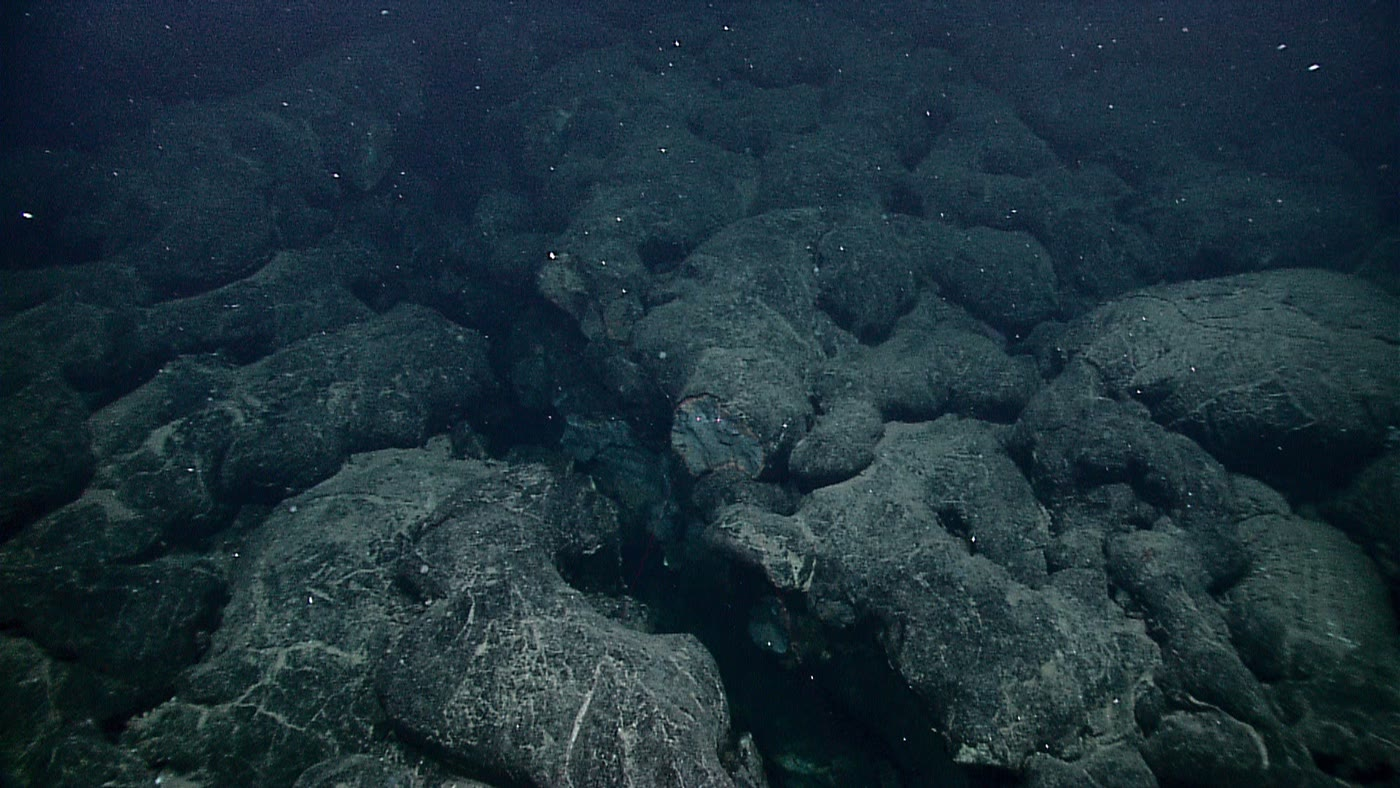
\includegraphics[width=0.6\linewidth]{images/book3/b1-pillow-lava.jpg}

\par\smallskip{\small \omterm{def:b1:rifts-ridges-margins:oceanic-crust}{Lavas en almohadillas} del rift de Galápagos, cortadas por una fisura que se abrió después de que se solidificaran: la
cima de la capa~2 de la \omterm{def:b1:rifts-ridges-margins:oceanic-crust}{corteza oceánica} en formación. Cada almohadilla es una lengua de lava congelada desde fuera por el agua de mar.
Fotografía: NOAA Okeanos Explorer Program, Galápagos Rift Expedition 2011, CC~BY~2.0 (Wikimedia Commons).}
\label{fig:b1:rifts-ridges-margins:pillows}
\end{omfigure}
% ledger: commons:pillow-expl6453

\begin{proposition}[Cada dique parte al anterior]\label{prop:b1:rifts-ridges-margins:dykes}
Supóngase que cada dique de un \omterm{def:b1:rifts-ridges-margins:oceanic-crust}{complejo de diques en enjambre} se intruye a lo largo del eje de expansión, donde la \omterm{def:b1:layered-earth:layers}{corteza} es más caliente
y débil, y que la \omterm{def:b1:layered-earth:layers}{corteza} se aleja del eje de forma simétrica. Entonces la mayoría de los diques se encuentran partidos en dos, cada mitad
con un margen enfriado solo contra su vecino más antiguo.
\end{proposition}

\begin{proof}
Un dique se enfría contra la roca más fría de ambos lados: tiene dos márgenes enfriados al formarse. El siguiente dique asciende donde la
\omterm{def:b1:layered-earth:layers}{corteza} es más débil, a lo largo del eje, es decir, por la mitad del anterior, aún la roca más caliente.
roca. Lo parte en dos mitades, que la expansión lleva a cada lado; cada mitad conserva el margen enfriado en su lado externo y tiene, en su
lado interno, el contacto sin enfriar con el dique nuevo. Todo dique excepto el último queda partido de esta manera.
\end{proof}

Los diques con un margen enfriado solo por un lado son, en efecto, la regla en los \omterm{def:b1:rifts-ridges-margins:oceanic-crust}{complejos de diques en enjambre}: la firma de una \omterm{def:b1:layered-earth:layers}{corteza}
construida, dique tras dique, por la expansión.


\section{La ley profundidad--edad}\label{sec:b1:rifts-ridges-margins:depth-age}

El fondo oceánico es somero en la dorsal y profundo lejos de ella. Como el fondo se forma en la dorsal y se aleja de ella, la distancia a la
dorsal es la edad, y la profundidad del fondo depende de su edad. La placa se enfría desde arriba a medida que envejece
(\cref{ch:b1:heat-budget}); la roca fría es más densa, y una columna más densa flota más abajo.

\begin{lemma}[Una integral de la función error]\label{lem:b1:rifts-ridges-margins:erfc}
Con $\operatorname{erfc} u = 1 - \operatorname{erf} u =
\frac{2}{\sqrt\pi}\int_u^\infty e^{-s^2}\,\mathrm ds$,
\[
  \int_0^\infty \operatorname{erfc} u \,\mathrm du = \frac{1}{\sqrt\pi}.
\]
\end{lemma}

\begin{proof}
La derivada de $\operatorname{erfc}$ es $-\frac{2}{\sqrt\pi}e^{-u^2}$. Integrando por partes en $[0, X]$,
\[
  \int_0^X \operatorname{erfc} u\,\mathrm du
  = \bigl[u \operatorname{erfc} u\bigr]_0^X + \frac{2}{\sqrt\pi}\int_0^X u\,e^{-u^2}\,\mathrm du
  = X\operatorname{erfc} X + \frac{1}{\sqrt\pi}\bigl(1 - e^{-X^2}\bigr).
\]
Para $X > 0$ y $s \ge X$, $e^{-s^2} \le (s/X)e^{-s^2}$, así que
$X\operatorname{erfc} X \le \frac{2}{\sqrt\pi}\int_X^\infty s\,e^{-s^2}\,\mathrm ds
= e^{-X^2}/\sqrt\pi$, que tiende a 0. Haciendo $X \to \infty$ se obtiene el
resultado.
\end{proof}

\begin{theorem}[Ley profundidad--edad]\label{thm:b1:rifts-ridges-margins:depth-age}
Supóngase que
\begin{enumerate}
  \item el \omterm{def:b1:layered-earth:layers}{manto} abandona la dorsal a la temperatura uniforme $T_m$, y la placa oceánica de edad $t$ es un semiespacio enfriado desde
        entonces desde su superficie, mantenida a $T_0$, con la difusividad térmica $\kappa$;
  \item la densidad de la roca enfriada es $\rho_m\bigl(1 + \alpha(T_m -
        T)\bigr)$, con $\rho_m$ la densidad del \omterm{def:b1:layered-earth:layers}{manto} a $T_m$ y
        $\alpha$ su coeficiente de dilatación térmica;
  \item cada columna está en equilibrio isostático sobre una \omterm{def:b1:isostasy-gravity:isostasy}{profundidad de compensación} situada bajo la capa enfriada, y el agua de mar
        tiene la densidad $\rho_w$.
\end{enumerate}
Entonces la profundidad del fondo marino de edad $t$ es
\[
  d(t) = d_r + C\sqrt t, \qquad
  C = \frac{2}{\sqrt\pi}\,\frac{\rho_m\,\alpha\,(T_m - T_0)\sqrt\kappa}{\rho_m - \rho_w},
\]
donde $d_r$ es la profundidad del eje de la dorsal. Esta es la \emph{ley profundidad--edad}\index{ley profundidad--edad} del fondo oceánico.
\end{theorem}

\begin{proof}
La temperatura en el semiespacio enfriado es
\[
  T(z, t) = T_0 + (T_m - T_0)\operatorname{erf}\frac{z}{2\sqrt{\kappa t}},
\]
con $z$ la profundidad bajo el fondo marino; esta solución de la ecuación del calor se admite aquí, como en \cref{ch:b1:heat-budget}, y se
deduce en el libro de tercer año universitario. Compárese la columna en la dorsal, formada por agua hasta $d_r$ y por \omterm{def:b1:layered-earth:layers}{manto} a $T_m$ debajo,
con la columna de edad $t$, formada por agua hasta $d$ y por la placa enfriada debajo, ambas hasta la \omterm{def:b1:isostasy-gravity:isostasy}{profundidad de compensación} $D$. Sus
masas por unidad de área son iguales:
\[
  \rho_w d_r + \rho_m (D - d_r) = \rho_w d + \int_0^{D-d}\rho_m\bigl(1 + \alpha(T_m - T)\bigr)\mathrm dz
  = \rho_w d + \rho_m (D - d) + \rho_m\alpha\int_0^{D-d}(T_m - T)\,\mathrm dz.
\]
Por tanto
\[
  (\rho_m - \rho_w)(d - d_r) = \rho_m\alpha\int_0^{D-d}(T_m - T)\,\mathrm dz.
\]
Como $T_m - T = (T_m - T_0)\operatorname{erfc}\bigl(z/2\sqrt{\kappa t}\bigr)$ es despreciable bajo la capa enfriada, la integral puede
extenderse hasta el infinito; con $u = z/2\sqrt{\kappa t}$ y \cref{lem:b1:rifts-ridges-margins:erfc},
\[
  \int_0^\infty (T_m - T)\,\mathrm dz = (T_m - T_0)\,2\sqrt{\kappa t}\int_0^\infty\operatorname{erfc}u\,\mathrm du
  = \frac{2}{\sqrt\pi}(T_m - T_0)\sqrt{\kappa t}.
\]
Dividiendo por $\rho_m - \rho_w$ resulta $d - d_r = C\sqrt t$.
\end{proof}

El agua importa: a medida que la placa se hunde, el agua llena el espacio sobre ella, y su peso la empuja aún más abajo. El coeficiente de
dilatación efectivo $\alpha\rho_m/(\rho_m - \rho_w)$ es mayor que $\alpha$ en un factor $3300/2300 \approx 1.43$.

Con $\alpha = \qty{3.2e-5}{K^{-1}}$, $T_m - T_0 = \qty{1350}{K}$, $\kappa = \qty{e-6}{m^2.s^{-1}}$, $\rho_m = \qty{3300}{kg.m^{-3}}$ y
$\rho_w = \qty{1000}{kg.m^{-3}}$, y el tiempo contado en millones de años ($\sqrt{\kappa\times\qty{1}{Myr}} = \qty{5618}{m}$), el teorema
da $C = \qty{393}{m.Myr^{-1/2}}$. Las constantes ajustadas por Parsons y Sclater a las profundidades del Pacífico norte y del Atlántico norte,
una vez retirados los sedimentos, son parecidas: $d_r \approx \qty{2500}{m}$ y $C \approx \qty{350}{m.Myr^{-1/2}}$, desde 0 hasta
\qty{70}{Myr}. Los valores de $\alpha$ y $T_m$ usados arriba son los de su modelo de placa para fondo antiguo, un \omterm{def:b1:layered-earth:layers}{manto} a
\qty{1350}{\degreeCelsius} y $\alpha = \qty{3.2e-5}{\per\degreeCelsius}$, inciertos en una quinta y en una tercera parte respectivamente,
así que la concordancia de 393 con 350 es tan buena como cabía esperar.
% ledger: parsons:plate-model, ps77:depth-age

\begin{example}[Fondo oceánico de 25 y 100 millones de años]\label{ex:b1:rifts-ridges-margins:depths}
Con $d = 2500 + 350\sqrt t$ (metros, $t$ en millones de años), el fondo de \qty{25}{Myr} yace a $2500 + 350\times5 = \qty{4250}{m}$, y el de
\qty{100}{Myr} a $2500 + 350\times10 = \qty{6000}{m}$. El fondo se hunde \qty{1750}{m} en sus primeros 25 millones de años, y solo
\qty{1750}{m} más en los 75 siguientes.
\end{example}
% ledger: parsons:plate-model

\begin{omfigure}
\begin{tikzpicture}
\begin{axis}[omrecord, omdepth, width=0.84\linewidth, height=6.6cm,
  xmin=0, xmax=13.6, ymin=2000, ymax=6800,
  xlabel={raíz cuadrada de la edad del fondo, $\sqrt t$ (\unit{Myr^{1/2}})},
  ylabel={profundidad (\unit{m})},
  yticklabel style={/pgf/number format/set thousands separator={}},
  legend style={font=\scriptsize, at={(0.02,0.03)}, anchor=south west, draw=none, fill=white, fill opacity=0.85, text opacity=1},
  legend cell align=left]
% computed in figdata/bachelor-1/depth_age.py; ledger: data:etopo1, data:b2-seafloor-age, parsons:plate-model
\addplot[name path=lo, draw=none, forget plot] table[x expr=sqrt(\thisrow{t}), y=q1] {figdata/out/bachelor-1-depth_age-bins.dat};
\addplot[name path=hi, draw=none, forget plot] table[x expr=sqrt(\thisrow{t}), y=q3] {figdata/out/bachelor-1-depth_age-bins.dat};
\addplot[black!12] fill between[of=lo and hi];
\addlegendentry{mitad central de las celdas}
\addplot[only marks, mark=*, mark size=1.1pt, black!70] table[x expr=sqrt(\thisrow{t}), y=median] {figdata/out/bachelor-1-depth_age-bins.dat};
\addlegendentry{profundidad mediana, intervalos de edad de 2 Myr}
\addplot[very thick, omProp] table[x expr=sqrt(\thisrow{t}), y=halfspace] {figdata/out/bachelor-1-depth_age-models.dat};
\addlegendentry{semiespacio, $2500 + 350\sqrt t$}
\addplot[thick, omDef, densely dashed] table[x expr=sqrt(\thisrow{t}), y=plate] {figdata/out/bachelor-1-depth_age-models.dat};
\addlegendentry{modelo de placa, $6400 - 3200\,e^{-t/62.8}$}
\draw[black!50, densely dotted] (axis cs:8.944,2000) -- (axis cs:8.944,6800);
\node[font=\scriptsize, anchor=north west, black!70] at (axis cs:8.944,2060) {\qty{80}{Myr}};
\node[font=\scriptsize, anchor=north west, black!70] at (axis cs:4.472,2060) {\qty{20}{Myr}};
\draw[black!50, densely dotted] (axis cs:4.472,2000) -- (axis cs:4.472,6800);
\end{axis}
\end{tikzpicture}

\par\smallskip{\small Profundidad del fondo oceánico frente a la raíz cuadrada de su edad. Cada punto es la profundidad mediana de las
celdas de un grado del océano mundial cuyo fondo cae en un intervalo de edad de dos millones de años (31\,538 celdas, más profundas que
\qty{1000}{m}); la banda gris contiene la mitad central de ellas. La ley del semiespacio es una recta en este gráfico. El fondo joven la
sigue de cerca; el fondo más antiguo yace por encima de ella, porque las celdas llevan sus sedimentos e incluyen montes submarinos y mesetas
volcánicas, y porque el fondo antiguo deja de hundirse (discontinua: el modelo de placa). Datos: ETOPO1 (NOAA) y las edades del fondo
oceánico de Seton y otros (2020).}
\label{fig:b1:rifts-ridges-margins:depth-age}
\end{omfigure}

La figura pone a prueba el teorema en todo el océano. Hasta unos \qty{20}{Myr} ($\sqrt t \approx 4.5$) las medianas yacen a unos cien metros de
la ley. Una recta ajustada a las medianas más jóvenes que \qty{70}{Myr} tiene una pendiente de solo \qty{250}{m.Myr^{-1/2}}: las profundidades
medidas son las de la superficie del sedimento, mientras que la ley da la profundidad de la cima de la \omterm{def:b1:layered-earth:layers}{corteza}, y la cubierta de sedimentos
se engrosa con la edad. Entre 60 y \qty{80}{Myr}, el fondo se aparta de la ley de la raíz cuadrada incluso después de retirar sus
sedimentos: se vuelve más somero que la ley y deja de hundirse. El modelo de placa, una placa de \qty{125}{km} de espesor cuya base se
mantiene a la temperatura del \omterm{def:b1:layered-earth:layers}{manto}, describe este aplanamiento: su profundidad tiende a unos \qty{6400}{m}, y su \omterm{def:b1:heat-budget:heat-flow}{flujo de calor} a una
constante, como si el calor se suministrara a la base de las placas antiguas por el \omterm{def:b1:layered-earth:layers}{manto} en convección. Ese modelo se estudia en el libro
de tercer año universitario; en este libro la ley de la raíz cuadrada se usa hasta \qty{80}{Myr}.
% ledger: parsons:plate-model; fit and cell count from depth_age.py (values part)

\begin{method}[Datación del fondo oceánico a partir de su profundidad]\label{met:b1:rifts-ridges-margins:age-from-depth}
Para estimar la edad del fondo oceánico donde sus anomalías magnéticas están ausentes o sin cartografiar:
\begin{enumerate}
  \item mídase la profundidad del fondo y, a partir de perfiles sísmicos, el espesor de sus sedimentos; tómese la profundidad $d$ de la
        cima de la \omterm{def:b1:layered-earth:layers}{corteza}, corregida por el peso de los sedimentos;
  \item inviértase la ley: $t = \bigl((d - d_r)/C\bigr)^2$, con $d_r$ y $C$ para
        el océano en cuestión;
  \item compruébese que el fondo es más joven que unos \qty{80}{Myr}, y estímese la incertidumbre: un error $\delta d$ en la profundidad da
        $\delta t = 2t\,\delta d/(d - d_r)$.
\end{enumerate}
\end{method}

Para un fondo a \qty{4600}{m}, $t = (2100/350)^2 = \qty{36}{Myr}$, y una incertidumbre de \qty{100}{m} en la profundidad da $2\times36\times100/2100 \approx
\qty{3.4}{Myr}$ en la edad. Donde el fondo es más somero que lo que predice la ley en una región amplia, un abombamiento, la causa no es la edad sino el
calor desde abajo (\cref{ch:b1:hotspots}).

La ley también enlaza el océano con el nivel del mar. Una dorsal que se expande más deprisa lleva el fondo joven y somero más lejos de su eje;
las cuencas oceánicas contienen menos agua, y el mar sube sobre los continentes. A lo largo de decenas de millones de años, los cambios de la
velocidad de expansión son una de las dos causas principales de los cambios del nivel global del mar, junto con el volumen de hielo en tierra.

\section{Fallas transformantes y zonas de fractura}

Las dorsales no son líneas continuas: están cortadas en segmentos desplazados por fallas que cruzan en ángulo recto, a lo largo de la dirección de
expansión. Más allá de los desplazamientos, las fallas continúan como largas cicatrices a través del fondo oceánico.

\begin{definition}[Falla transformante, zona de fractura]\label{def:b1:rifts-ridges-margins:transform}
Una \emph{falla transformante}\index{falla transformante} es una falla de desgarre que es una frontera de placas y termina en otras fronteras
de placas; una transformante dorsal--dorsal une los extremos de dos segmentos de dorsal desplazados. Una \emph{zona de fractura}\index{zona de fractura} es la prolongación de una falla transformante más allá de los extremos de los segmentos de dorsal: un valle o escalón lineal a través
del fondo oceánico que separa fondo de edades distintas que pertenece a una sola placa.
\end{definition}

\begin{proposition}[Deslizamiento en una transformante dorsal--dorsal]\label{prop:b1:rifts-ridges-margins:transform}
Dos segmentos de dorsal que se expanden simétricamente con la velocidad media $u$, perpendiculares a sí mismos, están desplazados por una
\omterm{def:b1:rifts-ridges-margins:transform}{falla transformante} de longitud $a$. Entonces:
\begin{enumerate}
  \item los dos lados de la transformante se deslizan uno junto a otro a la velocidad total $2u$, en el sentido opuesto al que sugeriría el
        desplazamiento si una sola dorsal recta hubiera sido cortada y desplazada por la falla;
  \item a lo largo de las \omterm{def:b1:rifts-ridges-margins:transform}{zonas de fractura} los dos lados no se mueven uno respecto del otro, y el fondo de los dos lados difiere en edad en $a/u$;
  \item la longitud de la transformante no cambia con el tiempo.
\end{enumerate}
\end{proposition}

\begin{proof}
Tómese el eje $x$ a lo largo de la transformante, hacia el este, y el eje $y$ hacia el norte, en el sistema de la dorsal. Sea el segmento
norte la recta $x = 0$, $y > 0$, y el sur $x = a$, $y < 0$ (el desplazamiento va hacia el este al ir hacia el sur); la transformante es el
segmento $0 < x < a$ de $y = 0$. La placa occidental $W$ yace al oeste de ambos segmentos y se mueve a $-u$ a lo largo de $x$; la placa
oriental $E$ yace al este de ambos y se mueve a $+u$.

(1) Justo al norte de la transformante, en $0 < x < a$, el fondo yace al este del segmento norte: pertenece a $E$ y se mueve hacia el este a
$u$. Justo al sur de ella, el fondo yace al oeste del segmento sur: pertenece a $W$ y se mueve hacia el oeste a $u$. El lado norte se mueve
hacia el este a $2u$ respecto del lado sur: visto desde cualquiera de los dos lados, el lado lejano se mueve a la derecha, y el deslizamiento
es dextrógiro (dextral). Una dorsal recta cortada por la falla, con su parte sur ahora al este de su parte norte, registraría en cambio un
desplazamiento levógiro (sinistral).

(2) Para $x > a$, ambos lados yacen al este de sus segmentos y pertenecen a $E$: se mueven juntos. A la distancia $x$ del segmento norte, el
fondo al norte de la \omterm{def:b1:rifts-ridges-margins:transform}{zona de fractura} tiene la edad $x/u$; el fondo al sur de ella está a $x - a$ del segmento sur y tiene la edad
$(x - a)/u$. La diferencia es $a/u$. Lo mismo vale para $x < 0$, donde ambos lados pertenecen a $W$.

(3) Ambos segmentos permanecen en $x = 0$ y $x = a$ en el sistema de la dorsal, ya que cada uno se expande simétricamente: la transformante
conserva la longitud $a$.
\end{proof}

J.\ Tuzo Wilson vio en 1965 que los desplazamientos de las dorsales no pueden leerse como el desplazamiento de una dorsal recta más antigua, y
predijo el sentido del deslizamiento de la proposición; los mecanismos focales de los terremotos en las transformantes lo confirmaron. Los
terremotos se producen a lo largo de la transformante activa, entre los extremos de la dorsal; las \omterm{def:b1:rifts-ridges-margins:transform}{zonas de fractura} suelen estar tranquilas.
A través de una \omterm{def:b1:rifts-ridges-margins:transform}{zona de fractura} el fondo de los dos lados tiene edades distintas, y por tanto, según la \omterm{thm:b1:rifts-ridges-margins:depth-age}{ley profundidad--edad}, profundidades
distintas: un escalón que se atenúa lentamente con la distancia a la dorsal. En el Atlántico norte, cerca de \ang{52}\,N, las dos
transformantes de Charlie--Gibbs desplazan la dorsal medioatlántica unos \qty{350}{km} en total.
% ledger: wilson:transform, data:pb2002 (offset summed over the transform steps in figdata/bachelor-1/ridge_budget.py)

\begin{omfigure}
\begin{tikzpicture}[x=0.95cm, y=0.95cm, font=\scriptsize]
\fill[omSea!10] (-5,-2.6) rectangle (8,2.6);
% isochrons (10 and 20 Myr), offset across the fracture zones
\foreach \x in {-4,-2,2,4} \draw[black!40] (\x,0) -- (\x,2.5);
\foreach \x in {-1,1,5,7} \draw[black!40] (\x,0) -- (\x,-2.5);
\node[black!55, anchor=south, fill=omSea!10, inner sep=1pt] at (2,2.0) {10};
\node[black!55, anchor=south, fill=omSea!10, inner sep=1pt] at (4,2.0) {20};
\node[black!55, anchor=south, fill=omSea!10, inner sep=1pt] at (-2,2.0) {10};
\node[black!55, anchor=south, fill=omSea!10, inner sep=1pt] at (-4,2.0) {20};
\node[black!55, anchor=north, fill=omSea!10, inner sep=1pt] at (5,-2.0) {10};
\node[black!55, anchor=north, fill=omSea!10, inner sep=1pt] at (7,-2.0) {20};
\node[black!55, anchor=north, fill=omSea!10, inner sep=1pt] at (1,-2.0) {10};
\node[black!55, anchor=north, fill=omSea!10, inner sep=1pt] at (-1,-2.0) {20};
% fracture zones and transform
\draw[black!60, thick, densely dashed] (-5,0) -- (0,0);
\draw[black!60, thick, densely dashed] (3,0) -- (8,0);
\draw[transform, line width=1.4pt] (0,0) -- (3,0);
% ridge segments
\draw[ridge, line width=1.1pt] (0,0) -- (0,2.6);
\draw[ridge, line width=1.1pt] (3,0) -- (3,-2.6);
\pic at (1.5,0) {dextral={90}};
\foreach \x in {0.4,0.75,2.25,2.6} \node[star, star points=5, star point ratio=2.2, fill=orange!90!black, draw=black, line width=0.2pt, inner sep=1.5pt] at (\x,0.0) {};
% plate motions
\draw[-{Stealth[length=4pt]}, very thick, black!70] (-2.8,1.1) -- (-3.9,1.1);
\draw[-{Stealth[length=4pt]}, very thick, black!70] (-0.2,-1.1) -- (-1.3,-1.1);
\draw[-{Stealth[length=4pt]}, very thick, black!70] (5.5,1.1) -- (6.6,1.1);
\draw[-{Stealth[length=4pt]}, very thick, black!70] (5.3,-1.1) -- (6.4,-1.1);
\node[font=\small] at (-3.3,1.55) {placa $W$};
\node[font=\small] at (6.1,1.55) {placa $E$};
\node[anchor=west, omRidge] at (0.1,2.25) {dorsal};
\node[anchor=east, omRidge] at (2.9,-2.25) {dorsal};
\node[anchor=north, align=center, fill=white, fill opacity=0.8, text opacity=1, inner sep=1pt] at (1.5,-0.35) {falla transformante\\(activa, terremotos)};
\node[anchor=south, fill=white, fill opacity=0.8, text opacity=1, inner sep=1pt] at (5.5,0.12) {zona de fractura (inactiva)};
\node[anchor=north, fill=white, fill opacity=0.8, text opacity=1, inner sep=1pt] at (-2.5,-0.12) {zona de fractura (inactiva)};
\node[anchor=south, black!70, fill=omSea!10, inner sep=1pt] at (6.2,0.55) {más antiguo, más profundo};
\node[anchor=north, black!70, fill=omSea!10, inner sep=1pt] at (6.0,-0.45) {más joven, más somero};
\end{tikzpicture}

\par\smallskip{\small Una dorsal desplazada por una \omterm{def:b1:rifts-ridges-margins:transform}{falla transformante}, en vista de mapa, con el norte arriba. Las dos placas se alejan de
cada segmento (flechas negras); a lo largo de la transformante (roja) se deslizan una junto a otra de forma dextrógira (semiflechas), aunque
el desplazamiento de la dorsal parezca levógiro. Las líneas grises son isócronas, marcadas en millones de años: a través de cada \omterm{def:b1:rifts-ridges-margins:transform}{zona de
fractura} (discontinua) el fondo de edades distintas, y por tanto de profundidades distintas, queda uno junto a otro, pero ambos lados se
mueven juntos. Estrellas: terremotos, confinados a la transformante.}
\label{fig:b1:rifts-ridges-margins:transform}
\end{omfigure}

Las transformantes son la tercera clase de evidencia de los movimientos de placas de \cref{ch:b1:plate-kinematics}: una transformante corre
a lo largo de la velocidad relativa de las dos placas, así que yace sobre un \omterm{def:b1:spherical-astronomy:spherical-triangle}{círculo menor} alrededor de su \omterm{def:b1:plate-kinematics:euler-pole}{polo de Euler}, y los \omterm{def:b1:spherical-astronomy:spherical-triangle}{círculos
máximos} trazados perpendiculares a varias transformantes se cortan en el polo. Las \omterm{def:b1:rifts-ridges-margins:transform}{zonas de fractura}, trazadas a través del fondo oceánico,
registran la dirección del movimiento en el pasado, como las anomalías magnéticas registran su velocidad.

\section{Ejercicios}

\begin{exercise}[$\star$]\label{exo:b1:rifts-ridges-margins:1}
En 2005 un segmento del rift de Afar de \qty{60}{km} de longitud se abrió hasta \qty{8}{m}, y se intruyeron \qty{2.5}{km^3} de magma. (a) Si el
dique hubiera tenido \qty{8}{m} de espesor a lo largo de todo el segmento, ¿cuál habría sido su altura media? (b) A la velocidad de placa de
\qty{18}{mm.yr^{-1}}, ¿cuántos años de movimiento representa una apertura de \qty{8}{m}?
% ledger: wright:afar, morvel:ar-nb
\end{exercise}

\begin{exercise}[$\star$]\label{exo:b1:rifts-ridges-margins:2}
Un \omterm{def:b1:rifts-ridges-margins:rift}{semigraben} está limitado por una falla de borde de salto \qty{3.0}{km} y \omterm{def:b1:geological-maps:attitude}{buzamiento} \ang{60}, y cortado por una falla antitética más pequeña
de salto \qty{0.8}{km} y \omterm{def:b1:geological-maps:attitude}{buzamiento} \ang{70}. (a) Calcúlese el \omterm{def:b1:cross-sections:throw}{salto horizontal} de cada falla y el estiramiento de la sección. (b) La sección
tiene ahora \qty{25}{km} de anchura: ¿cuánto medía antes del fallamiento?
\end{exercise}

\begin{exercise}[$\star$]\label{exo:b1:rifts-ridges-margins:3}
Clasifique las siguientes dorsales según los límites de la definición, a partir de sus \omterm{def:b1:plate-kinematics:spreading-rate}{velocidades de expansión totales} calculadas con
vectores de placa: dorsal de Gakkel \qty{12}{mm.yr^{-1}}; mar Rojo central \qty{15}{mm.yr^{-1}}; dorsal de Reykjanes
\qty{19}{mm.yr^{-1}}; dorsal de Carlsberg occidental \qty{23}{mm.yr^{-1}}; Atlántico Sur a \ang{20}\,S \qty{33}{mm.yr^{-1}}; dorsal del
Pacífico oriental a \ang{20}\,S \qty{143}{mm.yr^{-1}}. ¿Cuáles esperaría que tuvieran un valle axial, y cuáles un alto axial?
% ledger: morvel:eu-na, morvel:redsea, morvel:in-sm, morvel:nb-sa, morvel:nz-pa (rates computed with euler_velocities.py)
\end{exercise}

\begin{exercise}[$\star$]\label{exo:b1:rifts-ridges-margins:4}
Cada año se forman unos \qty{3.0}{km^2} de fondo oceánico nuevo, con una \omterm{def:b1:layered-earth:layers}{corteza} de \qty{7.1}{km} de espesor. (a) ¿Qué volumen de \omterm{def:b1:layered-earth:layers}{corteza} se
forma cada año? (b) A este ritmo, ¿cuánto tardaría en formarse el \qty{3.028e8}{km^2} del fondo oceánico? Compárese con la edad del fondo
oceánico más antiguo, unos \qty{190}{Myr}, y explíquese por qué ambos no tienen por qué coincidir.
% ledger: data:pb2002 (ridge_budget.py), white:crust, dd10:split, data:b2-seafloor-age
\end{exercise}

\begin{exercise}[$\star\star$]\label{exo:b1:rifts-ridges-margins:5}
Con $d = 2500 + 350\sqrt t$ (metros, $t$ en millones de años): (a) calcúlese la profundidad del fondo de 4, 36 y 64 millones de años;
(b) hállese la edad del fondo que yace a \qty{4600}{m} y a \qty{5300}{m}; (c) ¿cuánto se hunde el fondo entre 4 y \qty{36}{Myr}, y entre
36 y \qty{64}{Myr}?
\end{exercise}

\begin{exercise}[$\star\star$]\label{exo:b1:rifts-ridges-margins:6}
Calcúlese la constante $C$ de la \omterm{thm:b1:rifts-ridges-margins:depth-age}{ley profundidad--edad}
(\cref{thm:b1:rifts-ridges-margins:depth-age}) para $\alpha =
\qty{3.2e-5}{K^{-1}}$, $\rho_m = \qty{3300}{kg.m^{-3}}$, $\rho_w =
\qty{1000}{kg.m^{-3}}$, $T_m - T_0 = \qty{1350}{K}$ y $\kappa =
\qty{e-6}{m^2.s^{-1}}$, en \unit{m.Myr^{-1/2}}. Rehágase para un \omterm{def:b1:layered-earth:layers}{manto}
\qty{250}{K} más frío. ¿Qué constante seguiría el fondo de un océano más frío?
% ledger: parsons:plate-model
\end{exercise}

\begin{exercise}[$\star\star$]\label{exo:b1:rifts-ridges-margins:7}
El modelo de placa da el \omterm{def:b1:heat-budget:heat-flow}{flujo de calor} del fondo oceánico como $q = 11.3/\sqrt t$, en unidades de \qty{e-6}{cal.cm^{-2}.s^{-1}}, con $t$ en
millones de años. (a) Conviértase la constante a \unit{mW.m^{-2}.Myr^{1/2}} ($\qty{1}{cal} =
\qty{4.184}{J}$) y compárese con los \qty{490}{mW.m^{-2}.Myr^{1/2}} de \cref{ch:b1:heat-budget}. (b) Calcúlese $q$ a 1, 10 y \qty{150}{Myr}.
La ley se ajustó a fondo de hasta \qty{120}{Myr}, y el modelo de placa hace que el \omterm{def:b1:heat-budget:heat-flow}{flujo de calor} del fondo más antiguo se nivele en una
constante: ¿es el valor a \qty{150}{Myr} entonces demasiado alto o demasiado bajo?
% ledger: parsons:plate-model, dd10:young-ocean
\end{exercise}

\begin{exercise}[$\star\star$]\label{exo:b1:rifts-ridges-margins:8}
Una dorsal orientada norte--sur está cortada en dos segmentos; yendo hacia el sur a lo largo de la dorsal, el eje salta \qty{40}{km} hacia el
\emph{oeste} en una \omterm{def:b1:rifts-ridges-margins:transform}{falla transformante}. (a) ¿Cuál es el sentido del deslizamiento en la transformante? (b) ¿Qué parece mostrar el
desplazamiento de la dorsal? (c) ¿Dónde a lo largo de la línea de la transformante ocurren los terremotos, y por qué no más allá?
\end{exercise}

\begin{exercise}[$\star\star$]\label{exo:b1:rifts-ridges-margins:9}
Las \omterm{def:b1:rifts-ridges-margins:transform}{zonas de fractura} de Charlie--Gibbs desplazan la dorsal medioatlántica \qty{350}{km} en total; la \omterm{def:b1:plate-kinematics:spreading-rate}{velocidad de expansión total} allí es
\qty{21.2}{mm.yr^{-1}}. Trátese el desplazamiento como una sola transformante. (a) ¿Cuál es la diferencia de edad a través de la \omterm{def:b1:rifts-ridges-margins:transform}{zona de
fractura}? (b) Usando $d = 2500 + 350\sqrt t$, calcúlese el escalón de profundidad a través de la \omterm{def:b1:rifts-ridges-margins:transform}{zona de fractura} en el extremo de la
transformante, luego a \qty{100}{km} y a \qty{1000}{km} más allá de ella.
% ledger: data:pb2002 (ridge_budget.py), morvel:eu-na (rate at 52.5 N 31.5 W from euler_velocities.py)
\end{exercise}

\begin{exercise}[$\star\star\star$]\label{exo:b1:rifts-ridges-margins:10}
Una cuenca oceánica se forma a un ritmo constante y contiene fondo de todas las edades desde 0 hasta $A$ en áreas iguales. (a) Muéstrese
que su profundidad media es $d_r +
\frac23C\sqrt A$. (b) Con $d_r = \qty{2500}{m}$ y
$C = \qty{350}{m.Myr^{-1/2}}$, compárense $A = \qty{180}{Myr}$ y
$A = \qty{120}{Myr}$. (c) Si la expansión de la cuenca se acelera de modo que su fondo más antiguo tenga \qty{120}{Myr} en lugar de
\qty{180}{Myr}, ¿en cuánto sube el nivel del mar, despreciando la inundación de los continentes pero teniendo en cuenta la carga del agua
extra sobre el fondo, que se hunde $\rho_w/(\rho_m - \rho_w)$ veces la subida ($\rho_m = 3300$, $\rho_w = \qty{1000}{kg.m^{-3}}$)?
\end{exercise}

\begin{exercise}[$\star\star\star$]\label{exo:b1:rifts-ridges-margins:11}
En el marco de \cref{prop:b1:rifts-ridges-margins:transform}, el escalón de profundidad a través de una \omterm{def:b1:rifts-ridges-margins:transform}{zona de fractura} a la distancia $x > a$
del segmento de dorsal más lejano es $\Delta d = C\bigl(\sqrt{x/u} - \sqrt{(x - a)/u}\bigr)$. (a) Muéstrese que, para
$x \gg a$, $\Delta d \approx Ca/(2\sqrt{ux})$. (b) Con
$C = \qty{350}{m.Myr^{-1/2}}$, $a = \qty{350}{km}$ y
$u = \qty{10.6}{km.Myr^{-1}}$, compárense los escalones exacto y aproximado en
$x = 450$, 1350 y \qty{3350}{km}. ¿Cuándo es la aproximación buena hasta el
\qty{10}{\percent}?
\end{exercise}

\begin{exercise}[$\star\star\star$]\label{exo:b1:rifts-ridges-margins:12}
Compárese la ley del semiespacio $d_1(t) = 2500 + 350\sqrt t$ con la ley de placa $d_2(t) = 6400 - 3200\,e^{-t/62.8}$. (a) Calcúlese $d_2 - d_1$
a 10, 20, 30 y \qty{40}{Myr}. (b) Muéstrese que las dos leyes son iguales en una edad entre 20 y \qty{30}{Myr} y hállese con precisión de
\qty{0.1}{Myr} por bisección. (c) Compárense sus pendientes allí. ¿Por qué pueden empalmarse las dos leyes en esa edad sin una
discontinuidad visible?
% ledger: parsons:plate-model
\end{exercise}

\section{Problema: el nacimiento de un océano}

\begin{problem}[{Problema de fin de semana --- un continente estirado por sus fallas, un océano joven medido por sus franjas, y la
profundidad de su fondo a medida que envejece}]
\label{pb:b1:rifts-ridges-margins:1}
% values: calc/ch13.py (Part I rift section and Part II profile invented for the
% problem; real Euler vector, chron ages and depth--age constants)
% ledger: morvel:sm-an, morvel:nb-an, morvel:ar-nb, morvel:redsea, morvel:outward, iodp:gpts2004, heine:sam-saf, parsons:plate-model, wright:afar
Tómese $R = \qty{6371}{km}$. Un océano nace en tres etapas, cada una visible hoy en un lugar distinto: un \omterm{def:b1:rifts-ridges-margins:rift}{rift continental}, un océano
joven, un océano antiguo.

\medskip
\noindent\textbf{Parte I --- Un rift estirado por sus fallas.} Un corte a través de un rift orientado \ang{020} cruza seis fallas normales
cuyos saltos y \omterm{def:b1:geological-maps:attitude}{buzamientos} se midieron en perfiles sísmicos:
\begin{center}
\small
\begin{tabular}{lcccccc}
\hline
falla & F1 & F2 & F3 & F4 & F5 & F6\\
salto (\unit{m}) & 600 & 1100 & 2400 & 350 & 800 & 1500\\
\omterm{def:b1:geological-maps:attitude}{buzamiento} & \ang{60} & \ang{55} & \ang{50} & \ang{65} & \ang{60} & \ang{52}\\
\hline
\end{tabular}
\end{center}
Las fallas cortan lavas datadas en \qty{3.2}{Ma}, y el rift tiene ahora \qty{60}{km} de anchura.
\begin{enumerate}
  \item Calcúlese el \omterm{def:b1:cross-sections:throw}{salto horizontal} de cada falla. ¿Cuál es la falla de borde?
  \item Calcúlese el estiramiento de la sección y la anchura del rift antes del fallamiento.
  \item Las dos placas se separan a \qty{6.0}{mm.yr^{-1}} hacia \ang{105}. Calcúlese la componente de este movimiento perpendicular al rift.
  \item ¿Cuánto tardarían las placas en producir el estiramiento de la pregunta 2?
  \item ¿Cuánto se han separado las placas desde que se erupcionaron las lavas? ¿Qué fracción de ello lleva las fallas?
  \item Sugiera dónde ha ido el resto del estiramiento. Si se hubiera absorbido por diques como el de Afar en 2005, de \qty{8}{m} de anchura,
        ¿cuántos harían falta, y con qué frecuencia?
\end{enumerate}

\medskip
\noindent\textbf{Parte II --- Un océano joven medido por sus franjas.} Un perfil magnético a través del eje del mar Rojo central, en
\ang{18.0}\,N, \ang{40.0}\,E, sigue la dirección de expansión. El borde joven del cron C2An (\qty{2.581}{Ma}) yace a \qty{21.0}{km} al
noreste del eje y a \qty{20.2}{km} al suroeste de él; el borde antiguo del cron C3n (\qty{5.235}{Ma}) yace a \qty{41.0}{km} y
\qty{40.2}{km}. Los bordes de las anomalías están desplazados hacia fuera del eje \qty{2.2}{km} en total, de media, en ambos flancos.
\begin{enumerate}[resume]
  \item Calcúlese la \omterm{def:b1:plate-kinematics:spreading-rate}{velocidad de expansión total} a partir de cada cron, sin corregir.
  \item Corríjase cada velocidad por el desplazamiento hacia fuera. ¿Concuerdan las dos?
  \item Muéstrese que la velocidad calculada a partir de la distancia entre los dos crones de cada flanco no necesita corrección, y calcúlese.
  \item Calcúlense las velocidades medias en cada flanco a partir de las distancias entre los dos crones. ¿Es simétrica la expansión?
  \item El \omterm{def:b1:plate-kinematics:euler-pole}{polo de Euler} de Arabia respecto de Nubia está en \ang{30.9}\,N, \ang{23.6}\,E, con la velocidad \qty{0.403}{\degree\per\Myr}.
        Calcúlese la distancia angular del polo al perfil, y la velocidad total de expansión que predice allí el vector de placa.
  \item En el mar Rojo norte, a \ang{26.0}\,N, \ang{35.0}\,E, calcúlese la distancia angular al polo y la velocidad predicha.
  \item Compárense estas velocidades con las medidas, 15 y \qty{9}{mm.yr^{-1}}. ¿Por qué el mar Rojo se abre más deprisa en el sur?
\end{enumerate}

\medskip
\noindent\textbf{Parte III --- Hacia un Atlántico.}
\begin{enumerate}[resume]
  \item ¿Cuán ancho es el fondo oceánico formado en el mar Rojo central desde el borde antiguo de C3n, a la velocidad de la pregunta 9?
  \item El Atlántico Sur se abrió unos \qty{5000}{km} en Recife hace \qty{120.6}{Myr} (\cref{ch:b1:plate-kinematics}). Calcúlese su velocidad
        media de apertura.
  \item A la velocidad actual del mar Rojo central, ¿cuánto tardaría una apertura de \qty{5000}{km}? ¿Y a la velocidad del mar Rojo norte?
  \item El mar Rojo se abre alrededor de un polo cercano a él. ¿Qué implica esto para su forma a medida que se ensancha, y para el tiempo
        que necesita la parte norte para alcanzar la anchura que la parte central tiene ahora?
  \item ¿Qué tipo de dorsal es el eje del mar Rojo, y qué forma de eje espera?
\end{enumerate}

\medskip
\noindent\textbf{Parte IV --- El fondo se hunde.} Úsese $d = 2500 + 350\sqrt t$ (metros, $t$ en millones de años) y, para comparar, la ley de
placa $6400 - 3200\,e^{-t/62.8}$.
\begin{enumerate}[resume]
  \item Calcúlese la profundidad del nuevo fondo a las edades de 1, 10 y \qty{40}{Myr}.
  \item ¿A qué edad alcanza el fondo \qty{4000}{m}?
  \item El fondo junto a cada \omterm{def:b1:rifts-ridges-margins:passive-margin}{margen pasivo} tiene la edad del océano. ¿Cuánto se hunde en los primeros \qty{10}{Myr} tras la ruptura, y entre
        70 y \qty{80}{Myr}?
  \item ¿A qué velocidad, en metros por millón de años, se hunde ese fondo cuando el océano tiene \qty{80}{Myr}?
  \item ¿Qué \omterm{def:b1:heat-budget:heat-flow}{flujo de calor} pierde entonces el fondo de la pregunta 22, con $q = 490/\sqrt t$ en \unit{mW.m^{-2}}?
  \item Calcúlese la profundidad del fondo de \qty{80}{Myr} con cada una de las dos leyes, y su diferencia. ¿Por qué pueden compararse las dos a esta edad?
  \item Con precisión de una décima de kilómetro, ¿a qué profundidad sitúa la ley de la raíz cuadrada el fondo marino del océano nuevo cuando tiene 80 millones de años?
\end{enumerate}
\end{problem}
